\section{Observation and Calculations}

For this particular setup, we have measured $R_1 = 990$ $\Omega$ and $R_s = 195.9\,\Omega$. The diode resistance under reverse bias was measured to be $R_\text{diode} \approx 63$ M$\Omega$.

Hence $G$ comes out to be $3.216 \times 10^4$. The observed values of $V_1$ along with the corresponding temperature is given in Table \ref{tab}.

\begin{table}[]
    \centering
    \begin{tabular}{|c|c|c|c|c|c|}
    \hline
    $\theta\,(^\circ)$ & $t(\theta)$ (s) & $n(\theta)$ & $n_\text{avg}(\theta)$ & $N_d(\theta)$ (in s$^{-1}$) & $N(\theta)$ (in s$^{-1}$) \\ \hline
    \multirow{3}{*}{5} & \multirow{3}{*}{100} & 5082 & \multirow{3}{*}{5070.3} & \multirow{3}{*}{50.70} & \multirow{3}{*}{92.59} \\ \cline{3-3}
     &  & 5024 &  &  &  \\ \cline{3-3}
     &  & 5105 &  &  &  \\ \hline
    \multirow{3}{*}{10} & \multirow{3}{*}{100} & 2880 & \multirow{3}{*}{2885.0} & \multirow{3}{*}{28.85} & \multirow{3}{*}{26.44} \\ \cline{3-3}
     &  & 2912 &  &  &  \\ \cline{3-3}
     &  & 2863 &  &  &  \\ \hline
    \multirow{3}{*}{15} & \multirow{3}{*}{100} & 712 & \multirow{3}{*}{714.0} & \multirow{3}{*}{7.14} & \multirow{3}{*}{4.39} \\ \cline{3-3}
     &  & 693 &  &  &  \\ \cline{3-3}
     &  & 737 &  &  &  \\ \hline
    \multirow{3}{*}{20} & \multirow{3}{*}{200} & 220 & \multirow{3}{*}{230.7} & \multirow{3}{*}{1.15} & \multirow{3}{*}{0.54} \\ \cline{3-3}
     &  & 225 &  &  &  \\ \cline{3-3}
     &  & 247 &  &  &  \\ \hline
    \multirow{2}{*}{25} & \multirow{2}{*}{600} & 205 & \multirow{2}{*}{205.0} & \multirow{2}{*}{0.34} & \multirow{2}{*}{0.13} \\ \cline{3-3}
     &  & 205 &  &  &  \\ \hline
    \multirow{2}{*}{30} & \multirow{2}{*}{900} & 127 & \multirow{2}{*}{124.0} & \multirow{2}{*}{0.14} & \multirow{2}{*}{0.04} \\ \cline{3-3}
     &  & 121 &  &  &  \\ \hline
    \multirow{3}{*}{-5} & \multirow{3}{*}{100} & 5295 & \multirow{3}{*}{5278.3} & \multirow{3}{*}{52.78} & \multirow{3}{*}{96.39} \\ \cline{3-3}
     &  & 5281 &  &  &  \\ \cline{3-3}
     &  & 5259 &  &  &  \\ \hline
    \multirow{2}{*}{-10} & \multirow{2}{*}{100} & 3466 & \multirow{2}{*}{3492.0} & \multirow{2}{*}{34.92} & \multirow{2}{*}{32.01} \\ \cline{3-3}
     &  & 3518 &  &  &  \\ \hline
    \multirow{2}{*}{-15} & \multirow{2}{*}{100} & 947 & \multirow{2}{*}{953.5} & \multirow{2}{*}{9.54} & \multirow{2}{*}{5.86} \\ \cline{3-3}
     &  & 960 &  &  &  \\ \hline
    \multirow{2}{*}{-20} & \multirow{2}{*}{200} & 340 & \multirow{2}{*}{368.5} & \multirow{2}{*}{1.84} & \multirow{2}{*}{0.86} \\ \cline{3-3}
     &  & 397 &  &  &  \\ \hline
    \multirow{2}{*}{-25} & \multirow{2}{*}{600} & 252 & \multirow{2}{*}{261.0} & \multirow{2}{*}{0.44} & \multirow{2}{*}{0.16} \\ \cline{3-3}
     &  & 270 &  &  &  \\ \hline
    \multirow{2}{*}{-30} & \multirow{2}{*}{900} & 133 & \multirow{2}{*}{131.0} & \multirow{2}{*}{0.15} & \multirow{2}{*}{0.05} \\ \cline{3-3}
     &  & 129 &  &  &  \\ \hline
    \end{tabular}
    \caption{Measured counts $n$ for different scattering angles for Au foil of width 5mm. $N_d$ refers to counts per second. $N$ refers to the space corrected count rate as per Eq. \ref{eq:4}.}
    \label{tab}
    \end{table}

Fig. \ref{g} shows the plot between $\log(I_r)$ and $T^{-1}$. Using linear regression, we have obtained a best-fit straight line with slope and intercept as shown in the figure.

\begin{figure}
    \centering
    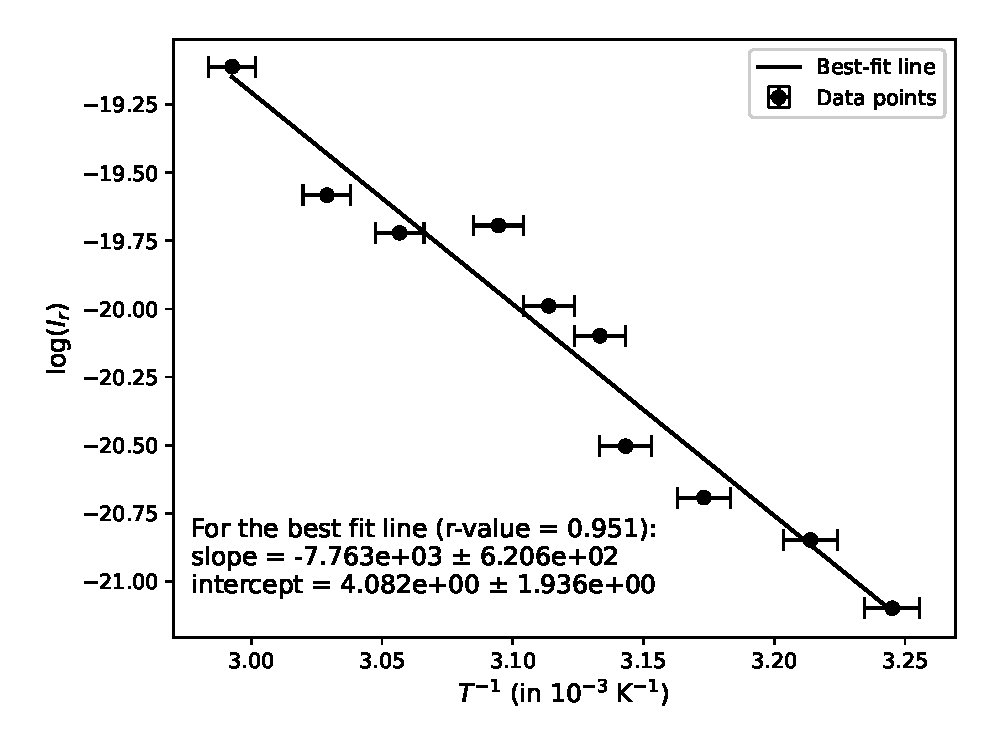
\includegraphics[width=1\columnwidth]{images/plot.eps}
    \caption{$\log(I_r)$ vs. $T^{-1}$ plot}
    \label{g}
\end{figure}

We can now use Eq. \ref{slope} to equate the slope and intercept to the corresponding physical parameters.

\begin{align*}
    m &= -7.763 \times 10^3 = -\frac{E_0}{\eta k_B}\\
    \implies E_0 &= 7.763 \times 10^3 \times \eta k_B\\
    &= 0.669 \text{ eV}
\end{align*}

\noindent using $k_B = 8.6173 \times 10^{-5}$ eV K$^{-1}$.
Similarly, we can also obtain
\begin{align*}
    c = 4.082 &= \ln(A)\\
    \implies A &= 59.27 \text{ Amp}
\end{align*}

For the purposes of this experiment, we do not discuss the value of $A$, which represents the \textit{reverse saturation current}.
\vspace{-1em}
\section{Error Analysis}

The error in $G$ can be derived from the error propagation formula using

\begin{align*}
    \Delta G &= \frac{R_\text{diode}\Delta R_s}{R_s^2} = 0.156 \nonumber
\end{align*}

\noindent using $\Delta R_s = 0.1\,\Omega$ and $\Delta R_\text{diode}/R_\text{diode} \approx 0$. The uncertainity in $I_r$ will be,

\begin{align}
    \frac{\Delta I_r}{I_r} = \sqrt{\left(\frac{\Delta V_1}{V_1}\right)^2 + \left(\frac{\Delta R_1}{R_1}\right)^2 + \left(\frac{\Delta G}{G}\right)^2}
\end{align}

\noindent $\Delta R_1 = 0.1\,\Omega$ and $\Delta V_1 = 10^{-8}$ A. Hence the uncertainity in $\ln(I_r)$ would be $\Delta I_r/I_r \sim 10^{-4}$ which is too small to be noticable in Fig. \ref{g}. The uncertainity in $T^{-1}$ is $\Delta T/T^2 \sim 10^{-5}$ where $\Delta T = 1^\circ$C.

Now, for the uncertainity in the band-gap, we get

\begin{align}
    \frac{\Delta E_0}{E_0} &= \sqrt{\left(\frac{\Delta \text{slope}}{\text{slope}}\right)^2}\\
    \implies \Delta E_0 &= 0.669 \times \frac{0.621}{7.763}\nonumber\\
    &= 0.053 \text{ eV}\nonumber
\end{align}